Calcolare (numericamente) la costante di Lebesgue per i polinomi interpolanti di grado $n = 2, 4, 6, ... , 40$, sia sulle ascisse equidistanti che su quelle di Chebyshev (utilizzare 10001 punti equispaziati per valutare la funzione di Lebesgue). Graficare convenientemente i risultati ottenuti. Spiegare, quindi, i risultati ottenuti approssimando la funzione
$$f(x)=\frac{1}{1+x^{2}},x\in[ - 5,5]$$
utilizzando le ascisse equidistanti e di Chebyshev precedentemente menzionate (tabulare il massimo errore valutato su una griglia di 10001 punti equidistanti nell’intervallo $[ - 5,5]$).

\hspace*{\fill}
\par\noindent\rule{\textwidth}{0.4pt}
\hspace*{\fill}

\textbf{Costante di Lebesgue}:
\lstinputlisting[language=Matlab]{Chapter-4/Exercise-19/lebesgue.m}
\textbf{Ascisse di Chebyshev}:
\lstinputlisting[language=Matlab]{Chapter-4/Exercise-19/ceby.m}
\begin{minipage}{\textwidth}
	\begin{lstlisting}[language=Matlab, caption=Codice Matlab]
	f = @(x) 1 ./ (1 + x.^2);
	a = -5;
	b = 5;
	n = 2 : 2 : 40;
	kxi = zeros(length(n), 1);
	kci = zeros(length(n), 1);
	x = linspace(a, b, 10001)';
	fx = f(x);
	ex = zeros(length(n), 1); ec = zeros(length(n), 1);

	figure(1)
	ax1 = subplot(2, 1, 1);
	for i = 1 : length(n)
		xi = linspace(a, b, n(i) + 1);
		fxi = f(xi);
		yxi = lagrange(xi, fxi, x);
		plot(ax1, x, yxi)
		hold on
		kxi(i, 1) = lebesgue(xi);
		ex(i) = norm(fx - yxi, inf);
	end
	legend('2', '4', '6', '8', '10', '12', '14', '16', '18', '20', '22', '24', '26', '28', '30', '32', '34', '36', '38', '40')
	hold off

	ax2 = subplot(2, 1, 2);
	for i = 1 : length(n)
		ci = ceby(n(i) + 1, a, b);
		x = linspace(min(ci), max(ci), 10001)';
		fx = f(x);
		fci = f(ci);
		yci = lagrange(ci, fci, x);
		plot(ax2, x, yci)
		hold on
		kci(i, 1) = lebesgue(ci);
		ec(i) = norm(fx - yci, inf);
	end
	legend('2', '4', '6', '8', '10', '12', '14', '16', '18', '20', '22', '24', '26', '28', '30', '32', '34', '36', '38', '40')
	hold off

	figure(2)
	plot(n, kxi, n, kci);
	legend('Ascisse equispaziate', 'Ascisse di Chebyshev')
	\end{lstlisting}
\end{minipage}

Le seguenti figure mostrano il polinomio di \textit{Lagrange}, al variare del grado \textit{n} del polinomio con $n=2,4,6,8...40$, utilizzando ascisse equidistanti e ascisse di Chebyshev:
\begin{figure}[H]
	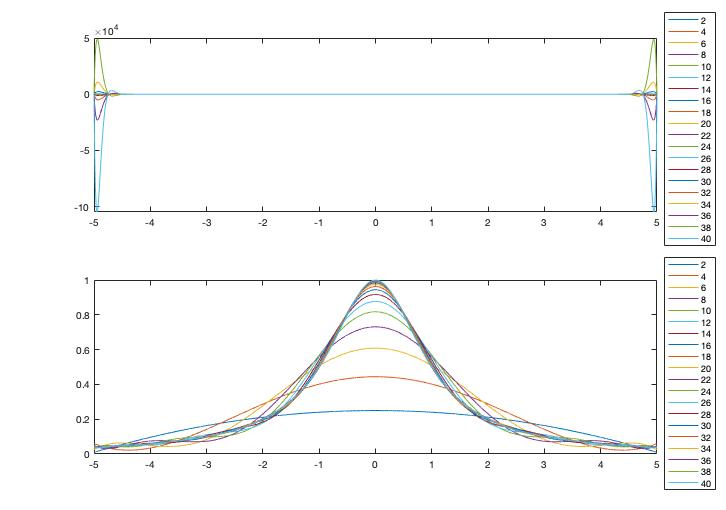
\includegraphics[width=\textwidth]{Chapter-4/Exercise-19/plot.jpg}
	\caption*{Polinomio di Lagrange con grado $n=2,4,6,8...40$, interpolante ascisse equidistanti e di Chebyshev}
\end{figure}
Nelle seguenti tabelle è riportato come varia la \textit{costante di Lebesgue} $\Lambda$, al variare del grado \textit{n} del polinomio e si può notare come la crescita sia \textit{esponenziale}, per $n\rightarrow\infty$, prendendo in cosiderazione \textit{ascisse equidistanti}:\\\
\begin{table}[H]
	\begin{minipage}{0.5\textwidth}
		\centering
		\caption{Costante di Lebesgue con ascisse equispaziate}
		\begin{tabular}{|c|c|}
			\hline
			$n$ & $\Lambda$ \\
			\hline
			$2$  & $1.250000000000000$ \\
			$4$  & $2.207824277504000$ \\
			$6$  & $4.549341110838356$ \\
			$8$  & $10.945005461386041$ \\
			$10$ & $29.898141093562188$ \\
			$12$ & $89.323735973507041$ \\
			$14$ & $2.831809493441890e+02$ \\
			$16$ & $9.342736404823136e+02$ \\
			$18$ & $3.170339307979169e+03$ \\
			$20$ & $1.097924392398584e+04$ \\
			$22$ & $3.866684343844037e+04$ \\
			$24$ & $1.378514896760509e+05$ \\
			$26$ & $4.964824917524024e+05$ \\
			$28$ & $1.802445465492321e+06$ \\
			$30$ & $6.592504744423425e+06$ \\
			$32$ & $2.430870357380395e+07$ \\
			$34$ & $8.978560703086898e+07$ \\
			$36$ & $3.348225693891219e+08$ \\
			$38$ & $1.249687039228850e+09$ \\
			$40$ & $4.678649708006595e+09$ \\
			\hline
		\end{tabular}
	\end{minipage}
	\hspace*{\fill}
	\begin{minipage}{0.5\textwidth}
		\centering
		\caption{Costante di Lebesgue con ascisse di Chebyshev}
		\begin{tabular}{|c|c|}
			\hline
			$n$ & $\Lambda$ \\
			\hline
			$2$  & $1.429872254730518e+00$ \\
			$4$  & $1.685135237733246e+00$ \\
			$6$  & $1.866863755668355e+00$ \\
			$8$  & $2.008324271512492e+00$ \\
			$10$ & $2.123677735937467e+00$ \\
			$12$ & $2.221698051371436e+00$ \\
			$14$ & $2.304741888790266e+00$ \\
			$16$ & $2.381233643402699e+00$ \\
			$18$ & $2.447573290086530e+00$ \\
			$20$ & $2.508706712856935e+00$ \\
			$22$ & $2.549521672833381e+00$ \\
			$24$ & $2.612618302290017e+00$ \\
			$26$ & $2.647525891619366e+00$ \\
			$28$ & $2.699620139181539e+00$ \\
			$30$ & $2.742631723381937e+00$ \\
			$32$ & $2.771163414194285e+00$ \\
			$34$ & $2.802963771799375e+00$ \\
			$36$ & $2.839252073343268e+00$ \\
			$38$ & $2.869838999732480e+00$ \\
			$40$ & $2.909700595498265e+00$ \\
			\hline
		\end{tabular}
	\end{minipage}
\end{table}

La seguente figura mostra in forma grafica i precedenti dati, espressi in forma tabellare:
\begin{figure}[H]
	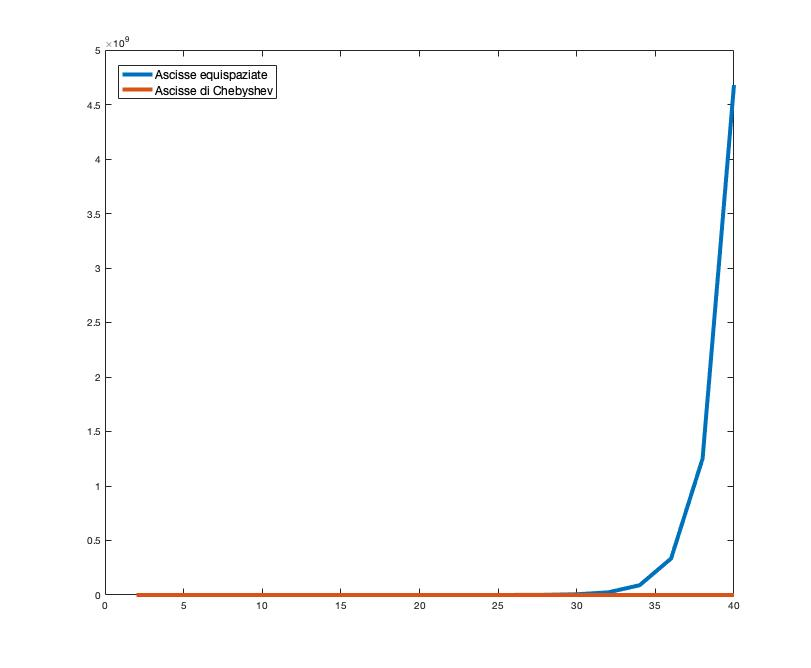
\includegraphics[width=\textwidth]{Chapter-4/Exercise-19/plot_lebesgue.jpg}
	\caption*{Crescita della costante di Lebesgue}
\end{figure}

Nelle seguenti tabelle viene invece riportato come varia il massimo errore di approssimazione, al variare del grado \textit{n} del polinomio:\\\
\begin{table}[H]
	\begin{minipage}{0.5\textwidth}
		\centering
		\caption{Massimo errore con ascisse equispaziate}
		\begin{tabular}{|c|c|}
			\hline
			$n$ & $Errore$ \\
			\hline
			$2$  & $6.462292487487394e-01$ \\
			$4$  & $4.383571218947540e-01$ \\
			$6$  & $6.169479236760332e-01$ \\
			$8$  & $1.045176501871859e+00$ \\
			$10$ & $1.915658802784827e+00$ \\
			$12$ & $3.663392805417856e+00$ \\
			$14$ & $7.194881107233104e+00$ \\
			$16$ & $1.439385128500340e+01$ \\
			$18$ & $2.919043772698086e+01$ \\
			$20$ & $5.982230871072865e+01$ \\
			$22$ & $1.236242551524645e+02$ \\
			$24$ & $2.572129123346204e+02$ \\
			$26$ & $5.381745497459237e+02$ \\
			$28$ & $1.131420473604506e+03$ \\
			$30$ & $2.388280971350734e+03$ \\
			$32$ & $5.058959841094824e+03$ \\
			$34$ & $1.074904570555982e+04$ \\
			$36$ & $2.290122855213777e+04$ \\
			$38$ & $4.890718541503938e+04$ \\
			$40$ & $1.046676859396163e+05$ \\
			\hline
		\end{tabular}
	\end{minipage}
	\hspace*{\fill}
	\begin{minipage}{0.5\textwidth}
		\centering
		\caption{Massimo errore con ascisse di Chebyshev}
		\begin{tabular}{|c|c|}
			\hline
			$n$ & $Errore$ \\
			\hline
			$2$  & $7.503001200480193e-01$ \\
			$4$  & $5.559113388123953e-01$ \\
			$6$  & $3.917402845902284e-01$ \\
			$8$  & $2.691783353450816e-01$ \\
			$10$ & $1.827582819736332e-01$ \\
			$12$ & $1.233976719701794e-01$ \\
			$14$ & $8.310704778474631e-02$ \\
			$16$ & $5.590747791183015e-02$ \\
			$18$ & $3.759032889290592e-02$ \\
			$20$ & $2.526854568700831e-02$ \\
			$22$ & $1.698393147777255e-02$ \\
			$24$ & $1.141498554193532e-02$ \\
			$26$ & $7.671902699208921e-03$ \\
			$28$ & $5.156161990762298e-03$ \\
			$30$ & $3.465357930583779e-03$ \\
			$32$ & $2.328996182090259e-03$ \\
			$34$ & $1.565269282134074e-03$ \\
			$36$ & $1.051984088923263e-03$ \\
			$38$ & $7.070159314990221e-04$ \\
			$40$ & $4.751701960865606e-04$ \\
			\hline
		\end{tabular}
	\end{minipage}
\end{table}

Dunque, possiamo osservare che avviene il cosiddetto \textbf{fenomeno di Runge}, ovvero un problema relativo all'interpolazione polinomiale su nodi equispaziati con polinomi
di grado elevato. È possibile provare che in tal caso l'errore di approssimazione tende all'infinito all'aumentare del grado del polinomio, anche osservando i risultati ottenuti.
Per evitare tale fenomeno, è necessario ricorrere all'utilizzo dei nodi di Chebyshev, oppure all'interpolazione tramite funzioni spline.
